\documentclass[
	10pt,								% globale Schriftgröße
	parskip=half-,						% setzt Absatzabstand hoch
	paper=a4,							% Format
	english,ngerman,					% lädt Sprachpakete
	]{scrartcl}							% Dokumentenklasse

% //////////////////// Pakete laden ////////////////////
\usepackage{amsmath}			% MUSS vor fontspec geladen werden
\usepackage{mathtools}			% modifiziert amsmath
\usepackage{amssymb}			% mathematische symbole, für \ceckmarks
\usepackage{amsthm}				% für proof
\usepackage{mathrsfs}			% für \mathscr
\usepackage{latexsym}
\usepackage{marvosym}				% für Lightning

\usepackage{fontspec} 			% funktioniert nur mit den neueren Compilern z.B. XeLaTeX
\usepackage{microtype}			% für bessere Worttrennung
\usepackage[ngerman]{babel} 	% Spracheinstellung
\usepackage{lmodern}			% verändert verwendete Schriftart, damit sie weniger pixelig ist

\usepackage{verbatim}
\usepackage{listings}			% Für Quellcode

\usepackage{graphicx}
\usepackage{tabularx}			% für Tabellen mit gleicher Spaltenbreite und automatischen Umbrüchen
\usepackage{fullpage}
\usepackage{multirow}			% für multirow in tabulars
\usepackage{rotate}
\usepackage[cmyk,table]{xcolor} % um Farben zu benutzen, kann mehr als das Paket color
\usepackage[					% Verlinkungen
	colorlinks,					% farbige Schrift, statt farbiger Rahmen
	linktocpage,				% verlinkt im Abb.Verzeichnis Seitenzahl statt Bildunterschrift
	linkcolor=blue				% setzt Farbe der Links auf blau
	]{hyperref}					% nur für digitale Anwendungen, url = "http://www.example.com"
\usepackage{url}				% für Webadressen wie e-mail usw.: "\url{http://www.example.com}"

\usepackage{enumerate}			% für versch. Aufzählungezeichen wie z.B. a)
\usepackage{xspace}				% folgt ein Leerzeichen nach einem \Befehl, wird es nicht verschluckt.
\usepackage{cancel}				% für das Durchstreichen u.a. in Matheformeln mit \cancel
\usepackage{float}              % zum Forcieren der Position von figure-Umgebungen

% zum Zeichnen (u.a. von Graphen)
\usepackage{fp}
\usepackage{tikz}
\usetikzlibrary{tikzmark}			% für \tikzmark{toRemember}
\usetikzlibrary{positioning}	% verbesserte Positionierung der Knoten
\usetikzlibrary{automata}		% für Automaten (GTI)
\usetikzlibrary{arrows}
\usetikzlibrary{shapes}
\usetikzlibrary{decorations.pathmorphing}
\usetikzlibrary{decorations.pathreplacing}
\usetikzlibrary{decorations.shapes}
\usetikzlibrary{decorations.text}

% //////////////////// Syntaxhighlighting ////////////////////
\lstloadlanguages{Python, Haskell, [LaTeX]TeX, Java}
\lstset{
   basicstyle=\footnotesize\ttfamily,	% \scriptsize the size of the fonts that are used for the code
   backgroundcolor = \color{bgcolour},	% legt Farbe der Box fest
   breakatwhitespace=false,	% sets if automatic breaks should only happen at whitespace
   breaklines=true,			% sets automatic line breaking
   captionpos=t,				% sets the caption-position to bottom, t for top
   commentstyle=\color{codeblue}\ttfamily,% comment style
   frame=single,				% adds a frame around the code
   keepspaces=true,			% keeps spaces in text, useful for keeping indentation
							% of code (possibly needs columns=flexible)
   keywordstyle=\bfseries\ttfamily\color{codepurple},% keyword style
   numbers=left,				% where to put the line-numbers;
   							% possible values are (none, left, right)
   numberstyle=\tiny\color{codegreen},	% the style that is used for the line-numbers
   numbersep=5pt,			% how far the line-numbers are from the code
   stepnumber=1,				% nummeriert nur jede i-te Zeile
   showspaces=false,			% show spaces everywhere adding particular underscores;
							% it overrides 'showstringspaces'
   showstringspaces=false,	% underline spaces within strings only
   showtabs=false,			% show tabs within strings adding particular underscores
   flexiblecolumns=false,
   tabsize=1,				% the step between two line-numbers. If 1: each line will be numbered
   stringstyle=\color{orange}\ttfamily,	% string literal style
   numberblanklines=false,				% leere Zeilen werden nicht mitnummeriert
   xleftmargin=1.2em,					% Abstand zum linken Layoutrand
   xrightmargin=0.4em,					% Abstand zum rechten Layoutrand
   aboveskip=2ex, 
}

\lstdefinestyle{py}{
   language=Python,
}
\lstdefinestyle{hs}{
   language=Haskell,
}
\lstdefinestyle{tex}{
	language=[LaTeX]TeX,
	escapeinside={\%*}{*)},     % if you want to add LaTeX within your code
	texcsstyle=*\bfseries\color{blue},% hervorhebung der tex-Schlüsselwörter
	morekeywords={*,$,\{,\},\[,\],lstinputlisting,includegraphics,
	rowcolor,columncolor,listoffigures,lstlistoflistings,
	subsection,subsubsection,textcolor,tableofcontents,colorbox,
	fcolorbox,definecolor,cellcolor,url,linktocpage,subtitle,
	subject,maketitle,usetikzlibrary,node,path,addbibresource,
	printbibliography},% if you want to add more keywords to the set
     numbers=none,
     numbersep=0pt,
     xleftmargin=0.4em,
}

\lstdefinestyle{java}{
	language=Java,
	extendedchars=true,		% lets you use non-ASCII characters;
   						% for 8-bits encodings only, does not work with UTF-8
}

\lstdefinelanguage[x64]{Assembler}     % add a "x64" dialect of Assembler
   [x86masm]{Assembler} % based on the "x86masm" dialect
   % with these extra keywords:
   {morekeywords={CDQE,CQO,CMPSQ,CMPXCHG16B,JRCXZ,LODSQ,MOVSXD, %
                  POPFQ,PUSHFQ,SCASQ,STOSQ,IRETQ,RDTSCP,SWAPGS, %
                  rax,rdx,rcx,rbx,rsi,rdi,rsp,rbp, %
                  r8,r8d,r8w,r8b,r9,r9d,r9w,r9b}
}					% for 8-bits encodings only, does not work with UTF-8

\lstdefinestyle{c}{
	language=c,
	extendedchars=true,		% for 8-bits encodings only, does not work with UTF-8
}

% //////////////////// eigene Kommandos ////////////////////
\newcommand\FU{Freie Universität Berlin\xspace}% benötigt package xspace
\newcommand\gdw{g.\,d.\,w.\xspace}
\newcommand\oBdA{o.\,B.\,d.\,A.\xspace}
\newcommand{\Eu}{\texteuro}
\newcommand\N{\mathbb{N}\xspace}
\newcommand\Q{\mathbb{Q}\xspace}
\newcommand\R{\mathbb{R}\xspace}
\newcommand\Z{\mathbb{Z}\xspace}
\newcommand\ohneNull{\ensuremath{\backslash\lbrace 0\rbrace}}% \{0}
\let\dhALT\dh	% Schreibt Befehl \dh in \dhALT um
\renewcommand\dh{d.\,h.\xspace}	%renew überschreibt command \dh
\newcommand\Bolt{\;\text{\LARGE\raisebox{-0.3em}{\Lightning}\normalsize}\xspace}% Blitz
\newcommand\zz{\ensuremath{\raisebox{+0.25ex}{Z}% zu zeigen
			\kern-0.4em\raisebox{-0.25ex}{Z}%
			\;\xspace}}
\newcommand{\from}{\ensuremath{\colon}}
\newcommand{\floor}[1]{\lfloor{#1}\rfloor}
\newcommand{\ceil}[1]{\lceil{#1}\rceil}
 \renewcommand{\L}{\ensuremath{\mathcal{L}}\xspace}
 \renewcommand{\P}{\ensuremath{\mathcal{P}}\xspace}
 \newcommand{\NL}{\ensuremath{\mathcal{N}\kern-0.2em\mathcal{L}}\xspace}
 \newcommand{\NP}{\ensuremath{\mathcal{NP}}\xspace}

% //////////////////// Mathefunktionen ////////////////////
\DeclareMathOperator{\Landau}{\mathcal{O}}
\DeclareMathOperator{\True}{True}
\DeclareMathOperator{\False}{False}

% //////////////////// eigene Theoreme ////////////////////
\newtheorem{theorem}{Satz}
\newtheorem{corollary}[theorem]{Folgerung}
\newtheorem{lemma}[theorem]{Lemma}
\newtheorem{observation}[theorem]{Beobachtung}
\newtheorem{definition}[theorem]{Definition}
\newtheorem{Literatur}[theorem]{Literatur}
% konfiguriert proof
\makeatletter
\newenvironment{Proof}[1][\proofname]{\par
  \pushQED{\qed}%
  \normalfont \topsep6\p@\@plus6\p@\relax
  \trivlist
  \item[\hskip\labelsep
%         \itshape
        \bfseries
    #1\@addpunct{.}]\ignorespaces
}{%
  \popQED\endtrivlist\@endpefalse
}
\makeatother

% //////////////////// eigene Farben ////////////////////
\let\definecolor=\xdefinecolor
\definecolor{FUgreen}{RGB}{153,204,0}
\definecolor{FUblue}{RGB}{0,51,102}

\definecolor{middlegray}{rgb}{0.5,0.5,0.5}
\definecolor{lightgray}{rgb}{0.8,0.8,0.8}
\definecolor{orange}{rgb}{0.8,0.3,0.3}
\definecolor{azur}{rgb}{0,0.7,1}
\definecolor{yac}{rgb}{0.6,0.6,0.1}
\definecolor{Pink}{rgb}{1,0,0.6}

\definecolor{bgcolour}{rgb}{0.97,0.97,0.97}
\definecolor{codegreen}{rgb}{0,0.6,0}
\definecolor{codegray}{rgb}{0.35,0.35,0.35}
\definecolor{codepurple}{rgb}{0.58,0,0.82}
\definecolor{codeblue}{rgb}{0.4,0.5,1}

% //////////////////// eigene Settings ////////////////////

\textheight = 230mm		% Höhe des Satzspiegels / Layouts
\footskip = 10ex			% Abstand zw. Fußzeile und Grundlinie letzter Textzeile
\parindent 0pt			% verhindert Einrückung der 1. Zeile eines Absatzes
\setkomafont{sectioning}{\rmfamily\bfseries}% setzt Ü-Schriften in Serifen, {disposition}											% bindet Header ein (WICHTIG)
\usepackage{graphicx}
\usepackage{listings} % inline code snippets

\newcommand{\dozent}{Prof.  Dr.  Agnès Voisard, Nicolas Lehmann}					% <-- Names des Dozenten eintragen
\newcommand{\tutor}{Hoffman Christian}						% <-- Name eurer Tutoriun eintragen
\newcommand{\tutoriumNo}{ 3, Gruppe 22}				% <-- Nummer im KVV nachschauen
\newcommand{\projectNo}{3. Iteration}									% <-- Nummer des Übungszettels
\newcommand{\veranstaltung}{Datenbank Systeme}	% <-- Name der Lehrveranstaltung eintragen
\newcommand{\semester}{SoeSe 2017}						% <-- z.B. SoSo 17, WiSe 17/18
\newcommand{\studenten}{Ingrid Tchilibou, Emil Milanov, Boyan Hristov}			% <-- Hier eure Namen eintragen


% /////////////////////// BEGIN DOKUMENT /////////////////////////


\begin{document}
% /////////////////////// BEGIN TITLEPAGE /////////////////////////
\begin{titlepage}
	\subject{\dozent}
	\title{\veranstaltung, \semester}
	\subtitle{\Large Project \projectNo\\ \large\vspace{1ex} TutorIn: \tutor\\ Tutorium \tutoriumNo}
	\author{\studenten}
	\date{\normalsize \today}
\end{titlepage}

\maketitle								% Erstellt das Titelblatt
\vspace*{-10cm}							% rückt Logo an den oberen Seitenrand
\makebox[\dimexpr\textwidth+1cm][r]{	%rechtsbündig und geht rechts 1cm über Layout hinaus
	
\includegraphics[width=0.4\textwidth]{src/fu_logo} % fügt FU-Logo ein
}
% /////////////////////// END TITLEPAGE /////////////////////////

\vspace{7cm}							% Abstand
\rule{\linewidth}{0.8pt}				% horizontale Linie										% erstellt die Titelseite

\section*{Allgemein}
Link zum Projekt: \url{https://github.com/gancia-kiss/dbs_projekt}


\section*{1. Aufgabe: Data Mining: Clustering}

\begin{enumerate}

\item Ähnlichkeitsmetrik

Um die gemeinsamkeit je 2 Hashtags zu berechnen, haben wir zwei Metriken genommen. Erstens ist es für uns wichtig, wie oft zwei Hashtags gemeinsam zusammen vorkommen und zweitens, wie oft diese in der selben Woche benutzt werden. So können wir beide Hashtags mit equivalente Bedeutungen als auch zu einander offensive Hashtags zusammenfassen. Wenn es ein Trend in einer Woche gibt, dann werden alle zu diesem Trend relevante Hashtags in der selben Woche benutzt, aber nicht unbedingt zusammen, da oft nur ein Paar Hashtags per Tweet benutzt werden, und nicht alle, die zu dem Thema relevant sind. Wenn zwei Hashtags aber doch nur zusammen vorkommen, muss das als eine stärkere Bindung markiert werden, deswegen reicht das Datum alleine nicht.

\item Clustering

Wir haben jede Woche und jeden Hashtag aus dem Datenbank eine eigene Dimension zugewiesen, damit wir diese in einem Vektorraum representieren können. Falls zum Beispiel ein Hashtag nur in der ersten und zweiten Woche verwendet wurde und zwar 2 mal in der ersten und 4 mal in der zweiten, dann sieht sein Vektor folgendermaßen aus \[[2,4,0,0,0...]\]Wenn man dann die Dimensionen für die Zusammenverwendung von Hashtags hinzufügt, und zum Beispiel unser Beispielshashtag der lexikographisch erste ist und nur zusammen mit dem 4. Hashtag 3 mal vorgekommen ist, dann sieht sein Vektor folgendermaßen aus \[[2,4,0,0,...,3,0,0,3,0,0,...,0]\]

So werden Hashtags, die in der selben Wochen benutzt werden, in der selben Dimensionen zusammen wachsen und folglich ein kürzeres Euklidischen Abstand haben. Das selbe gilt auch für die Zusammenverwendung im selben Tweet.

\item Curse of Dimensionality

Wir könnte aber leider ohne weiteres K-Means nicht erfolgreich auf der so konstruierten Vektorraum verwenden. Das liegt daran, dass unsere Daten in einer so großen Anzahl von Dimensionen sehr Sparse werden und dabei den euklidischen Abstand zwischen den enzigen Elemente stark abnimmt, so dass wir am Ende ein rießengroßen Cluster bekommen, wo fast alle Hashtags gesammelt werden, da diese nicht mehr so deutlich von einander unterscheidbar sind.

Als in der Bücher erklärt, wächst zusammen mit der Anzahl von Dimensionen auch der Anteil von Kantenlängen eines Hyperwürfels, um bestimmten Anteil des Hyperwürfels abzudecken. Damit nimmt die Ähnlichkeit im Sinne von euklidischen Abstand zwischen der einzelnen Punkte mit der Anzahl von Dimensionen drastisch ab. Deswegen werden im unserem Fall mehrere Punkte im selben Cluster gesammelt, obwohl die eigentlich nicht so nah sein dürfen.

Quellen: \\
Machine Learning: A Probabilistic Perspective, K.P. Murphy, 2012, S.18 \\
Deep Learning, I. Goodfellow, Y. Bengio, A. Courville, 2016, S. 151 \\
\url{https://en.wikipedia.org/wiki/Curse_of_dimensionality}

\item Lösung 
Wir haben Dimensionality Reduction verwandt, um die Punkte wieder näher zu bringen, damit wir erfolgreich K-Means anwenden können. Wir haben uns für den t-SNE ('t-distributed stochastic neighbor embedding') Algorithmus entschieden, der ein nicht-lineares Machine-Learning Algorithmus ist und die Ähnlichkeit der einzelnen Punkte bei der Reduktion versucht zu behalten. \\

Da aber zwei Dimensionen nicht ausreichbar sind, um unseren Daten richtig und verlustlos zu representieren, haben wir uns entschieden, erstmal nur auf 10 Dimensionen den Vektorraum zu reduzieren, K-Means anzuwenden und erst danach weiter auf 2 Dimensionen zu reduzieren für die Representierung. Dabei ist nicht mehr wichtig, dass alle Abstände richtig sind, da wie die Kantenbreite benutzen, um Ähnlichkeit zwischen je zwei Hashtags zu äußern.

Weiter haben wir für die Implementierung die Bibliothek Numpy benutzt, um leichter und deutlich effizienter Euklidische Abstände berechnen zu können, was wichtig für den K-Means Algorithmus ist. Wir haben dann alle Clusters, Kanten und Koordinaten von den Hashtags in beiden 10-Dimensionalen und 2-Dimensionalen Vektorraum in dem Datenbank gespeichert, damit wir leichter das Ergebniss analysieren können, bevor wir die Front-end Seite fertig gemacht haben.  



\end{enumerate}

\section*{2. Aufgabe: Datenvisualisierung}

\begin{enumerate}

\item Visualisierung von dem Clustering

Für den 'Maximum bang for the buck' haben wir für die Front-End Seite AngularJS zusammen mit Bootstrap genommen, da beide minimale Konfiguration erfordern und gute Leistung anbieten. AngularJS hat uns geholfen eine modernere Single-Page-Application entwickeln zu können und leichter Daten aus unserer API auf der HTML Seiten visualizieren zu können, mit Hilfe von Templates und 2-way-data-binding. Die Architektur ist natürlich für großere Projekten nicht so effizient, für unsere kleine Anwendung finden wir aber die Entscheidung ganz gut. Bootstrap ist ein CSS Framework, dass uns erlaubt hat, fast kein CSS zu schreiben und trotzdem schönes Endergebniss zu bekommen, damit sehen auch alle unsere UI Elemente einheitlich aus. \\

Wir haben gesehen, dass die Bibliothek 'SigmaJS' leicht mit JSON Dateien arbeitet, deswegen hatten wir keine Schwierigkeiten die Daten, die wir schon in dem Datenbank gespeichert haben, über Ajax Anfragen zu den Klient zu transportieren. \\ 

Für die Visualisierung haben wir uns entschieden, stärkere Beziehungen zwischen Hashtags mit dickeren Kanten darzustellen. Dabei wurde schon ein Constraint in der Aufgabenstellung gegeben, und nämlich das zwei Hashtags, die nie mit einander zusammen benutzt wurden, nicht mit einer Kante verbindet sein dürfen. Wir haben ein weiteres Constraint eingefügt, dass das auch für zwei Hashtags gilt, die sich nicht in dem selben Cluster befinden. Die verschiedene Farben bezeichnen bei uns auch die verschiedene 7 Cluster.

\item Visualisierung von der Häufigkeit

Für die Visualisierung der Häufigkeit haben wir die Bibliothek Mathplotlib benutzt. Wir haben schon in der letzten Projektiteration eine Tabelle eingeführt, wo gespeichert wird, in welchen Wochen ein Hashtag benutzt wurde und wie oft. Anhand von der existierenden Implementierung haben wir das selbe auch für die einzelne Tage gemacht und dann anhand davon die Visualisierung gemacht. Da wir auch eine Tabelle für die Wochen haben, haben wir den Nutzer die Möglichkeit gegeben, die gewünschte Einheit zu wählen.

\end{enumerate}

\section*{Anpassung des ER-Diagramms und damit auch des Datenbanks}

Wir haben noch alle für die Clusters und ihre Visualisierung benötigte Daten in dem Datenbank gespeichrt, damit wir die Antowrtzeit (Response-Time) des Servers minimieren. Das ER-Diagramm sieht jetzt folgedermaßen aus

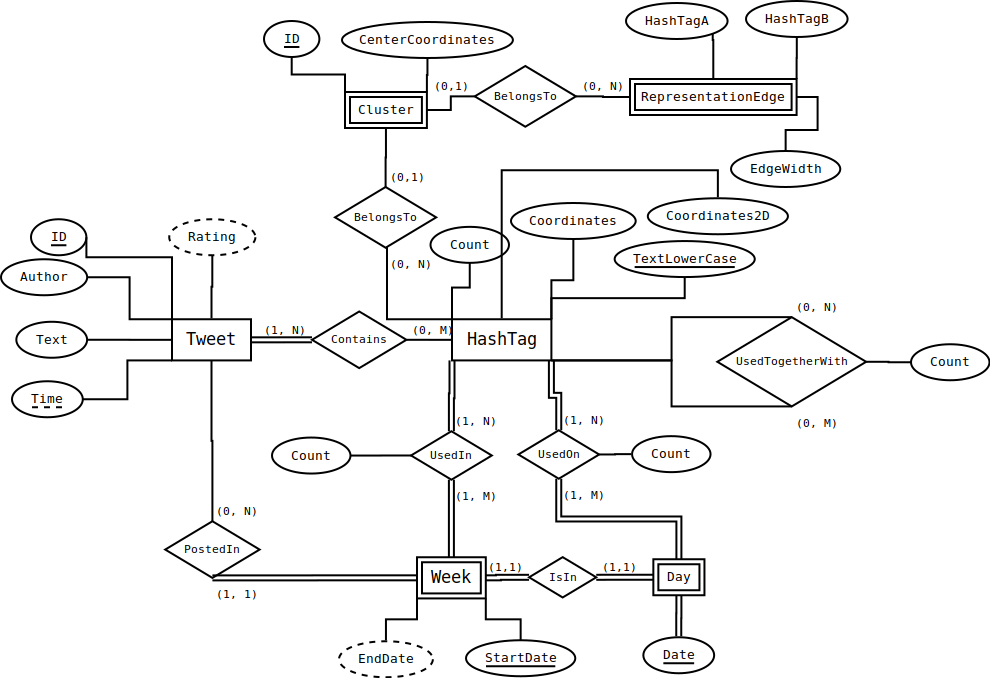
\includegraphics[width=\textwidth]{../ER-Diagramms/ERDiagramm_v2.png}

\section*{Schwierigkeiten}

Die größte Schwierigkeiten, die wir in dem Projekt hatten, waren bei der Clustering

\begin{enumerate}

\item Ersten Ansatz, Idee nicht realisiert

Wir haben am Anfang gedacht, dass wir das absolut minimalste Abstand zwischen alle Daten, in den zwei Hashtags benutzt wurden, nehmen können und dazu gegen proportional die Anzahl der Zusammenverwendungen nehmen können und dann die zwei Werte einfach skalieren und aufsummieren können. Die Idee ist für Abstandsberechnung ganz gut, damit kann man aber die Hashtags nicht in einem Vektorraum ordnen und dafür kann man auch K-Means in der Situation nicht anwenden.

\item Zweiten Ansatz

Wir haben dann die Hashtags richtig in einem n-dimensionalen Vektorraum geordnet, dabei aber keine Dimensionsreduktion gemacht. Dabei haben wir über 'Curse of dimensionality' gelernt. Die Clusters, die dabei entstanden sind, waren nur für die Hashtags gut, die ganz oft verwendet wurden, die nicht so berühmte aber wurden alle zu dem selben Cluster zugeordnet.

\item Dritten Ansatz

Wir haben Dimensionsreduktion angewandt und einigermaßen gute Clusters bekommen

\item Vierten Ansatz

Wir haben weiter gelesen, wie wir den t-SNE Algorithmus besser konfigurieren können, wie wir die zwei Features gut skalieren können und wie viele Clusters wir erstellen sollen. Die richtige Werte für die meisten dieser 'Tweaks' haben wir experimentell gefunden. Für die Skalierung des Gewichts der einzige Features haben wir überlegt, dass eine Kombination von 2 Hashtags in einem Tweet 2 mal in usedTogetherWith markiert wird und nur einmal in dem Datum, weiter gibt es auch deutlich mehrere Hashtags (damit auch Dimensionen dafür) als Wochen. Deswegen haben wir die Dimensionen für die Wochen mit 3 skaliert.

\end{enumerate}


\section*{Screenshots}

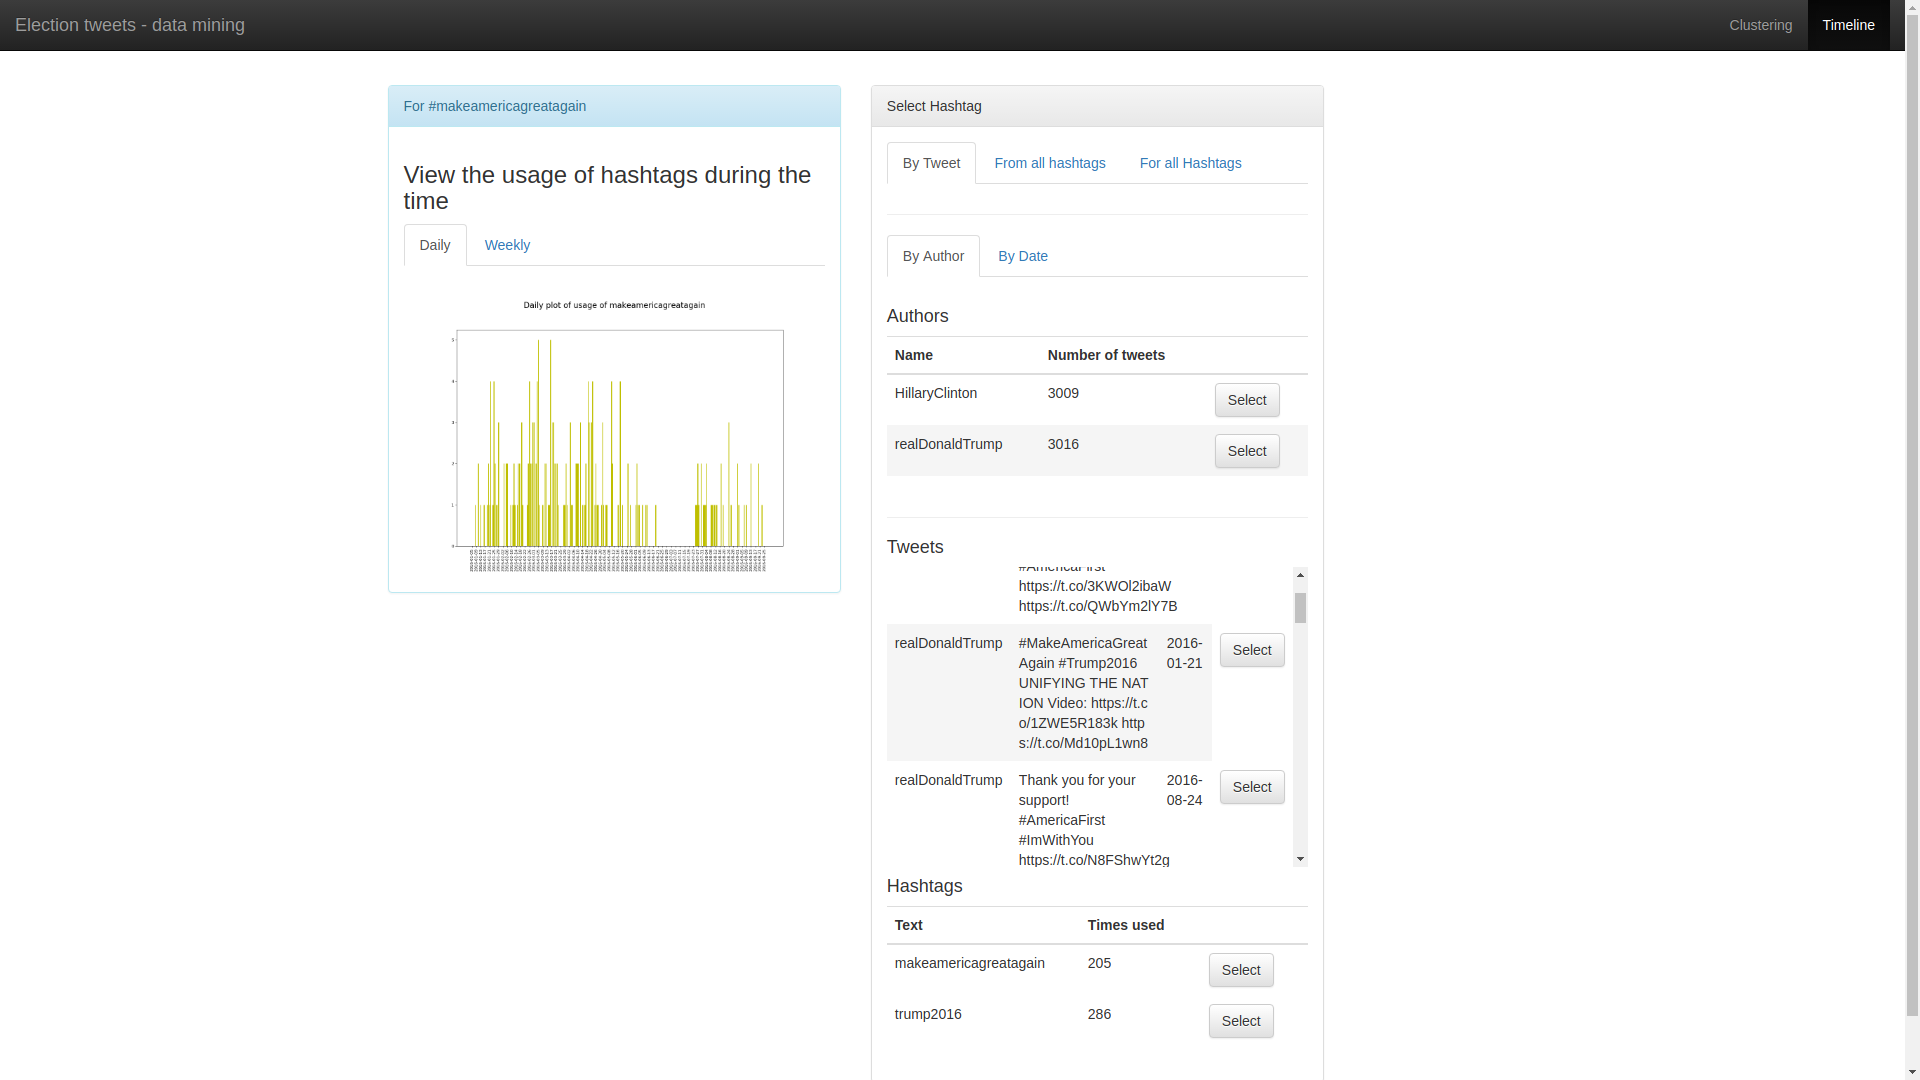
\includegraphics[width=\textwidth]{../Screenshots/a.png} \\ \\
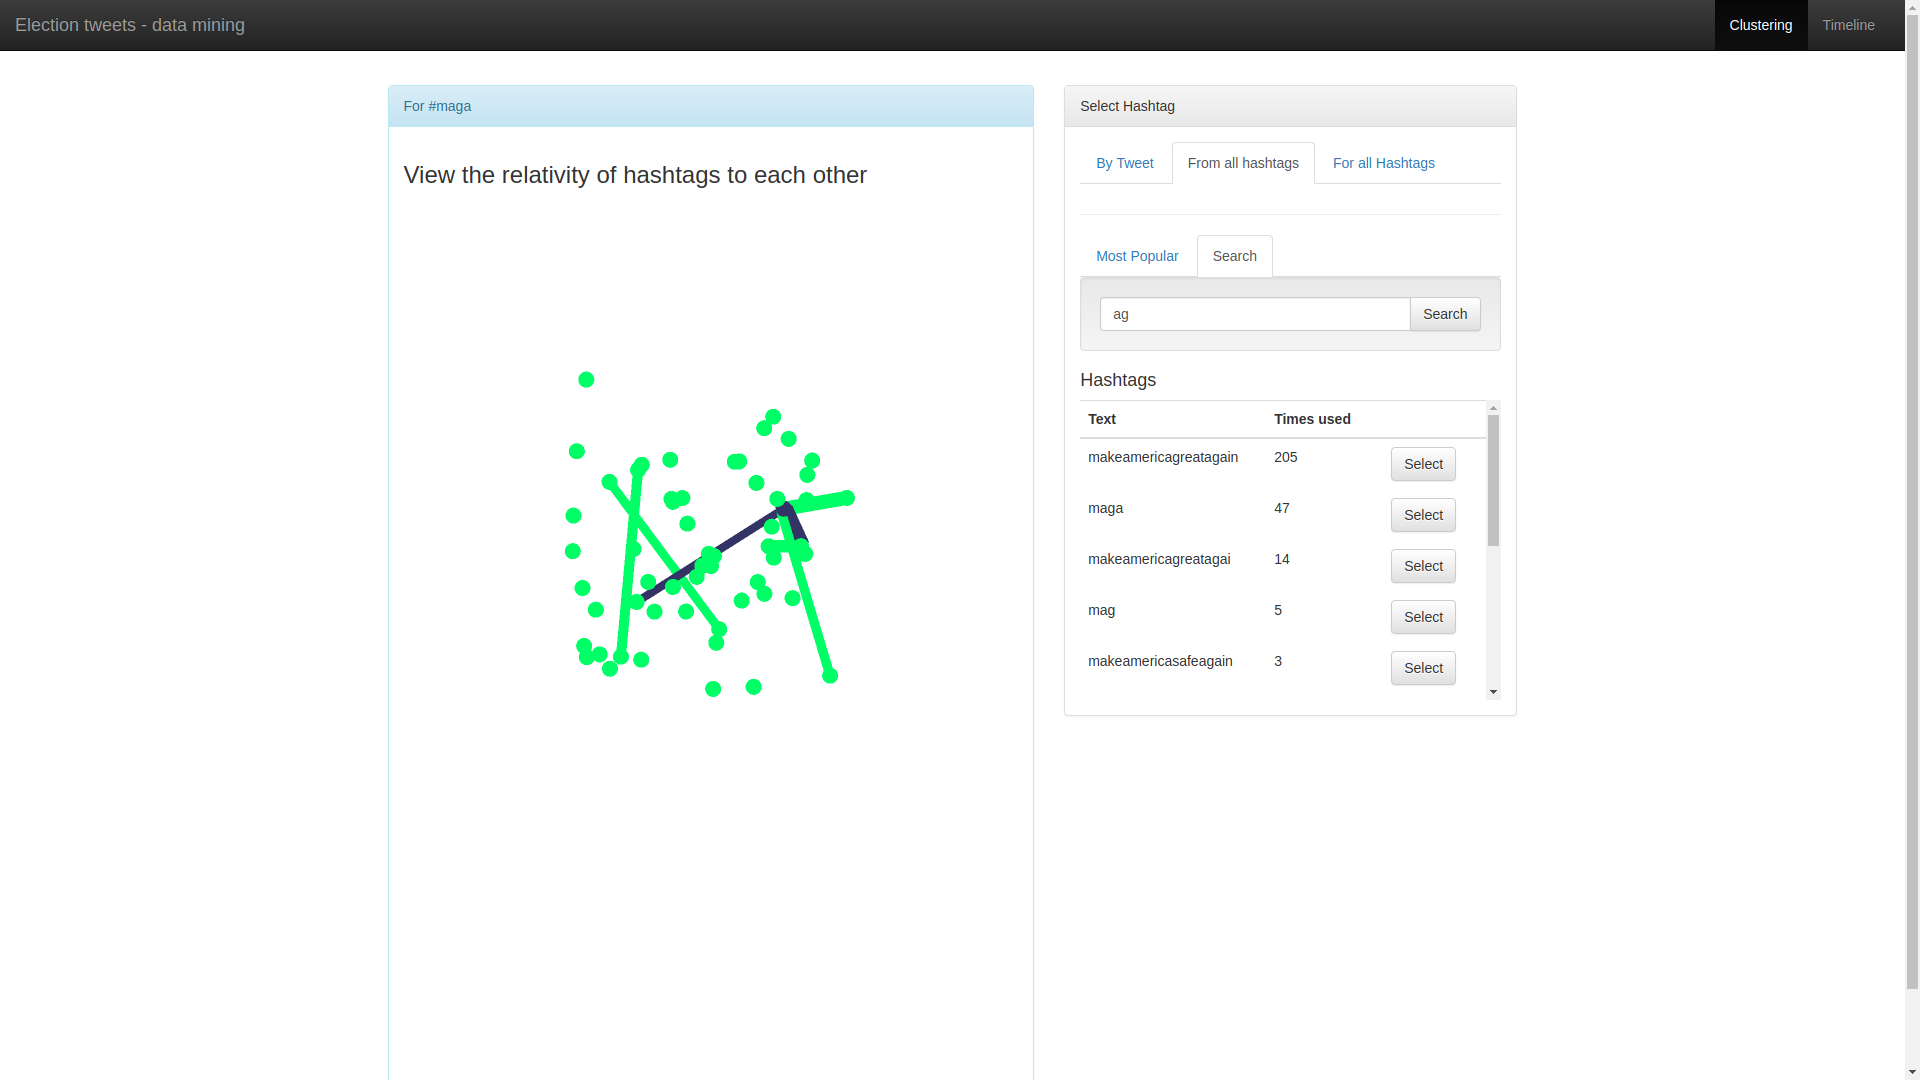
\includegraphics[width=\textwidth]{../Screenshots/b.png} \\ \\
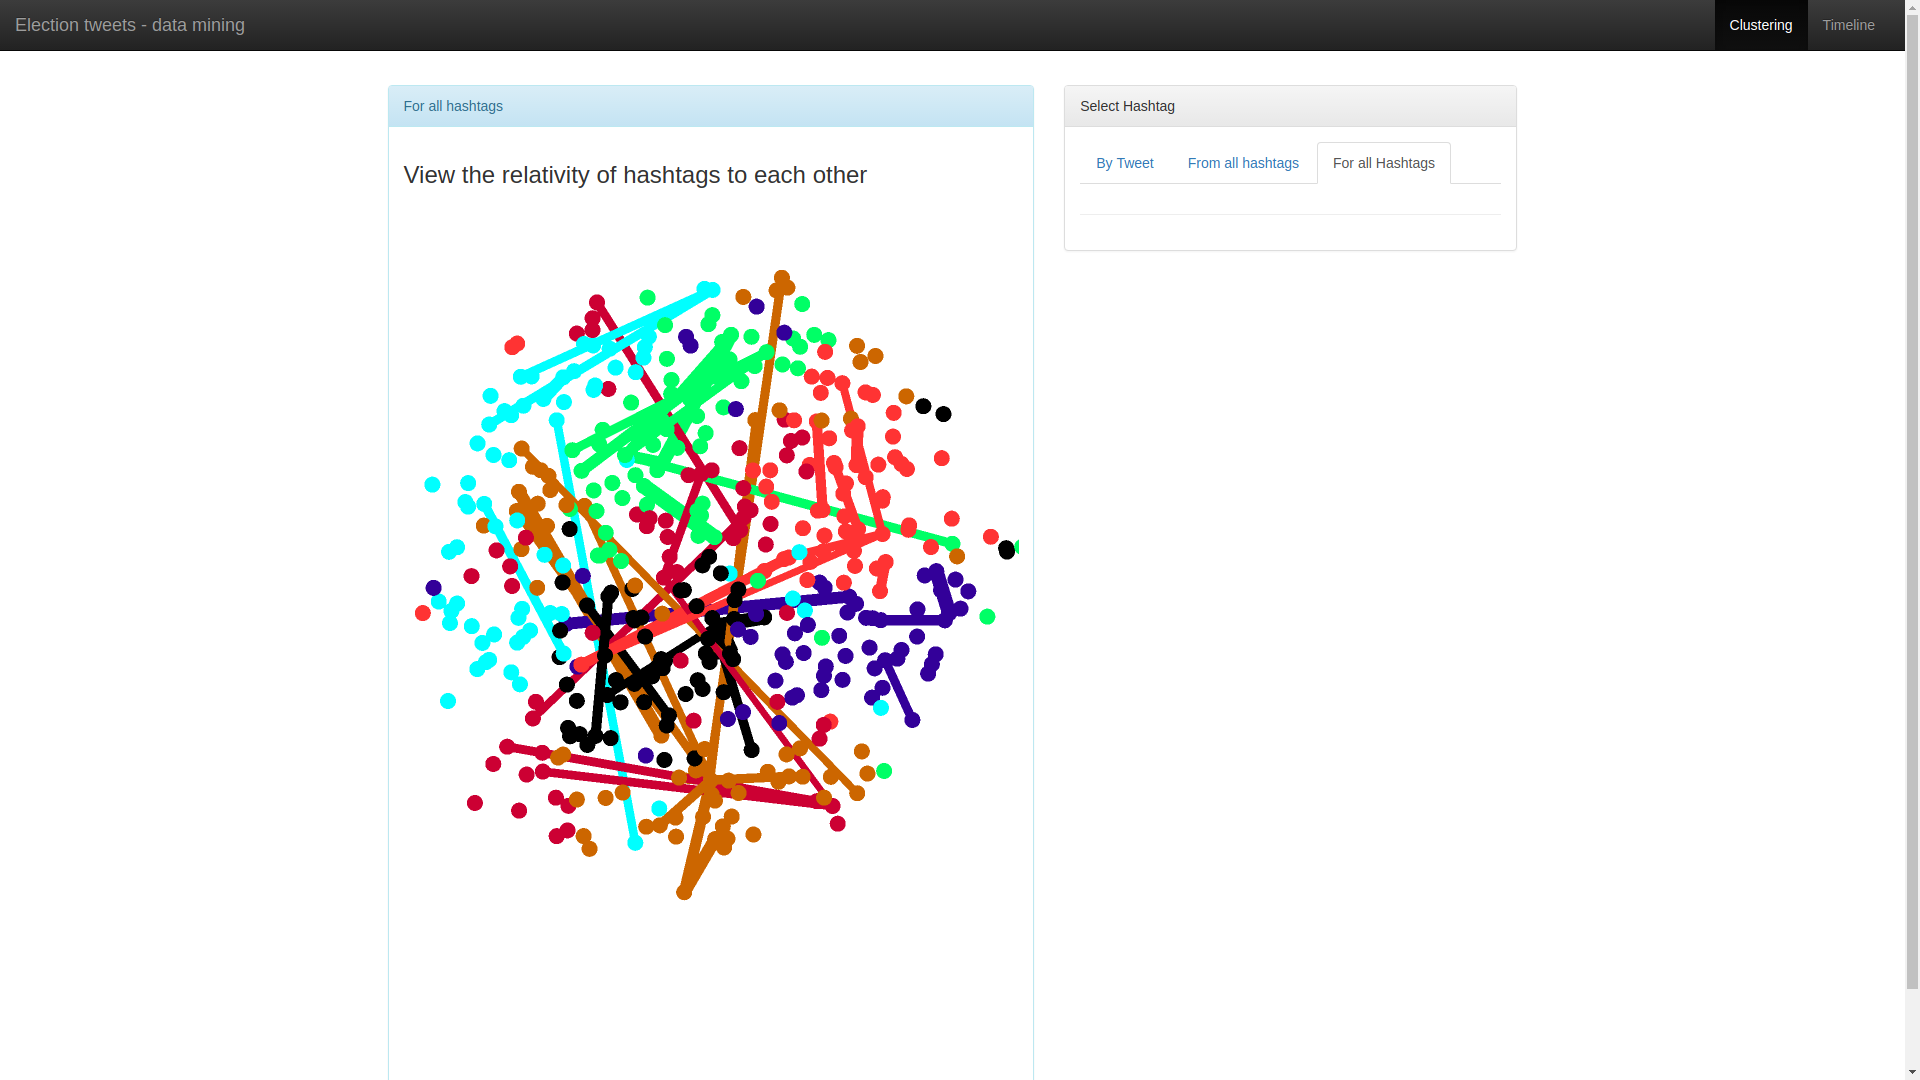
\includegraphics[width=\textwidth]{../Screenshots/c.png} \\ \\
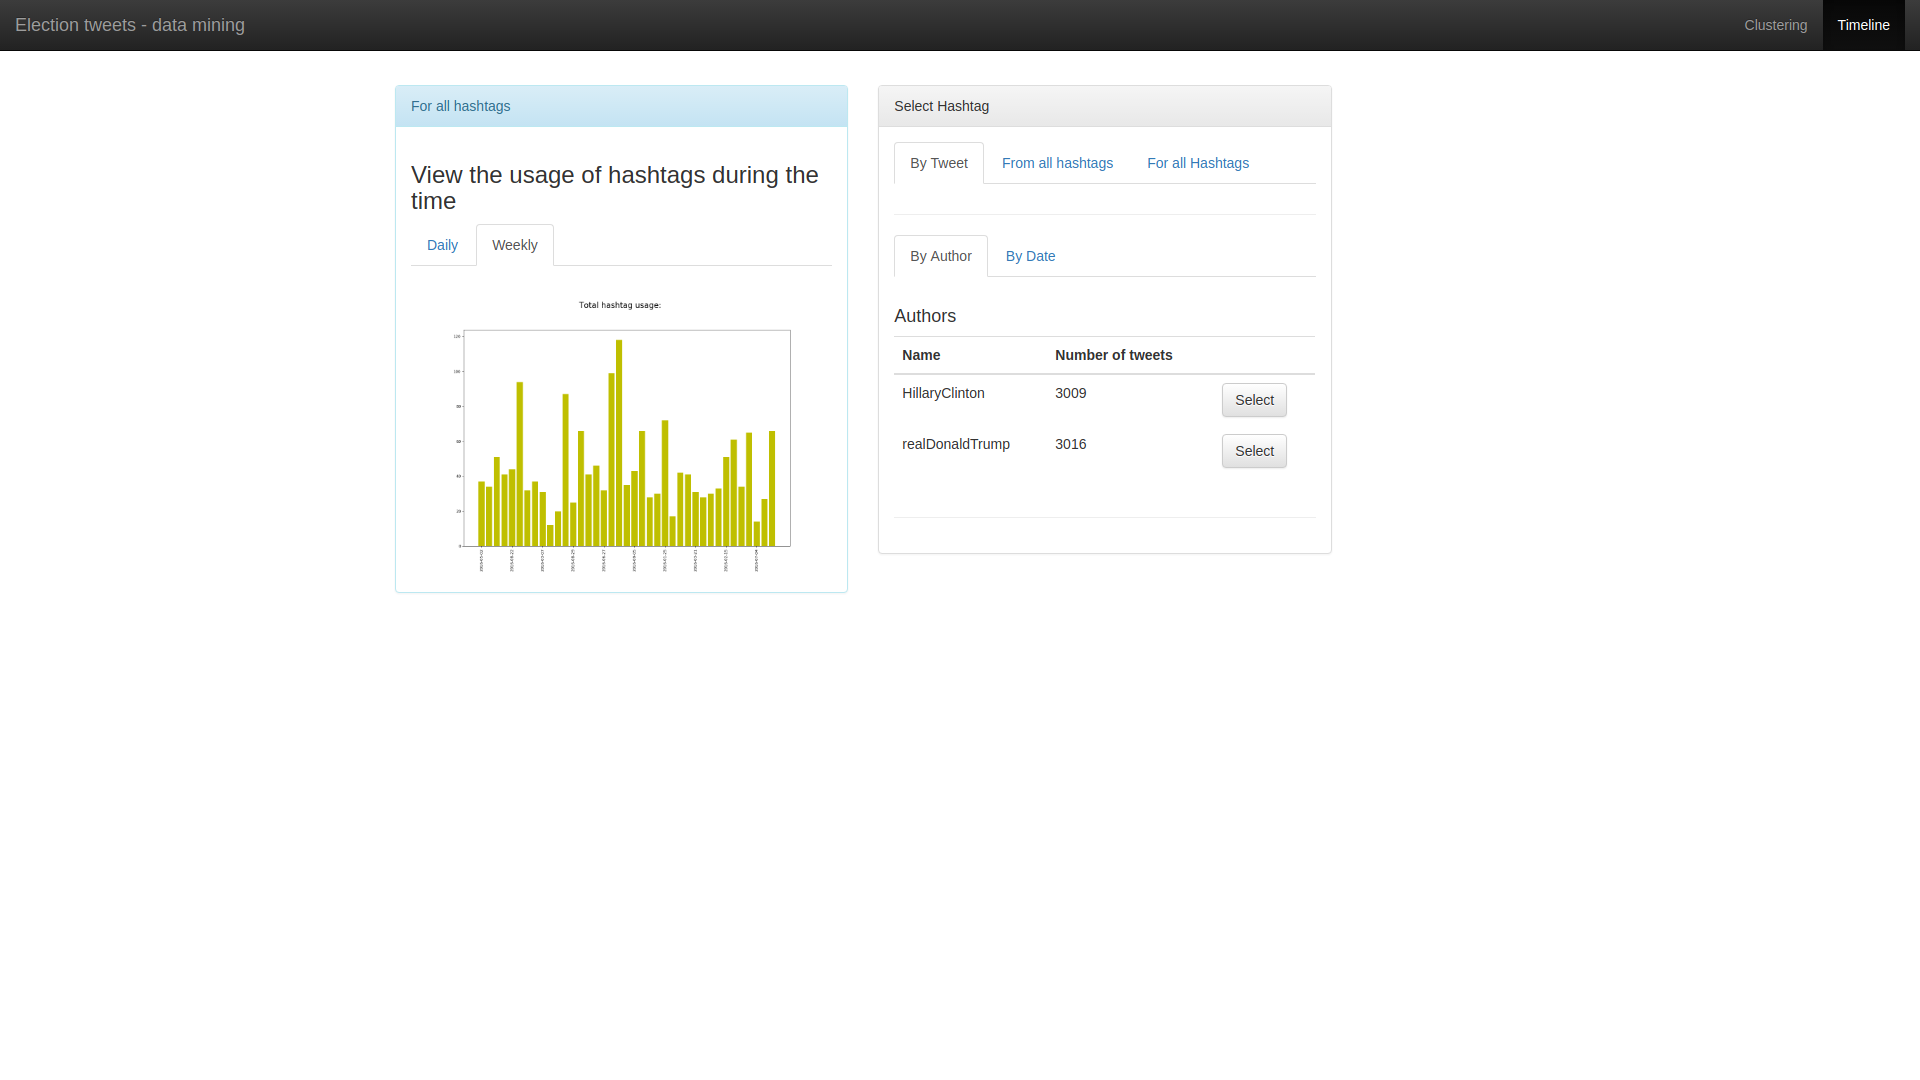
\includegraphics[width=\textwidth]{../Screenshots/d.png}

\end{document}
